\documentclass{beamer}
\usepackage{amsmath, amssymb}
\usepackage{bm}
\usepackage{luatexja}
\usepackage{mathrsfs}              % 花文字
\usepackage{multirow}              % 表結合
\usepackage{float}                 % 図の位置制御
\usepackage{url}                   % URL表示
\usepackage{type1cm}               % フォント調整
\usepackage{here}                  % H位置指定
\usepackage{physics}               % 量子力学向け記法
\usepackage{graphicx}
\usepackage{multicol}
\title{量子ドット内の電子状態の数値計算\\ ~ ハイブリッドポテンシャルによる解析と差分法 ~}
\author{}
\date{}

\begin{document}

\frame{\titlepage}

\begin{frame}{目次}
\tableofcontents
\end{frame}

\section{本演習の目的}
\begin{frame}{1. 本演習の目的}
この演習では、\textbf{半導体量子ドット中の電子状態}を、解析的および数値的手法を用いて解明することを目的とする。

対象は、\textbf{InSb材料により形成された円形の2次元量子ドット}。電子はこの中に閉じ込められ、ポテンシャル井戸の中でエネルギー準位が離散化される。

\begin{center}
  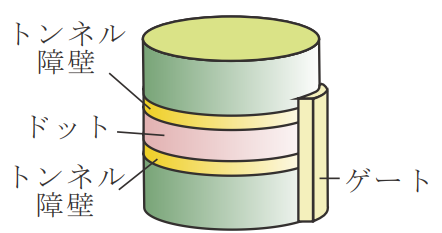
\includegraphics[width=0.4\textwidth]{images/ドット.png}
  
  図2.1:InSb 量子ドット構造
\end{center}
\end{frame}

\section{量子ドット}
\begin{frame}{2. 量子ドット}
量子ドットとは、電子の量子力学的な性質を顕著に引き出す\textbf{人工的な原子様構造}。

\begin{itemize}
\item \textbf{電子数を1個単位で制御できる}
\item \textbf{波動性が顕著になるサイズ(10〜100 nm)}
\end{itemize}

\medskip
応用例:
\begin{itemize}
\item 単一電子トランジスタ、量子ビット
\item 発光素子、レーザー
\end{itemize}

\begin{flushright}
  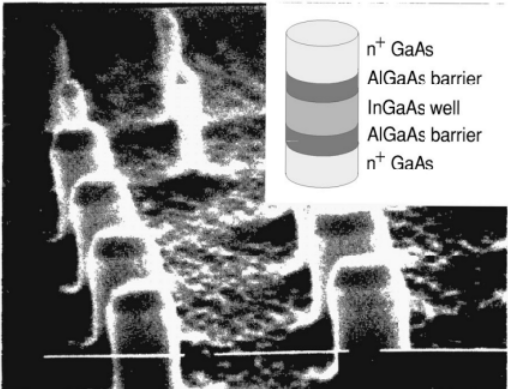
\includegraphics[width=0.3\textwidth]{images/量子ドット.png}\\
  図1:量子ドット
\end{flushright}
\end{frame}

\section{仮定と近似}
\begin{frame}{3. 仮定と近似}
本演習では、以下の仮定・近似を導入:

\begin{itemize}
\item \textbf{ハイブリッドポテンシャルの導入}
\item \textbf{有効質量近似と有効原子単位系}
\end{itemize}
\end{frame}

\begin{frame}{3.2 有効質量近似と定式化}
\textbf{有効質量近似}により、電子の運動は以下のように記述される:

\[
\left[ -\frac{\hbar^2}{2 m^*} \nabla^2 + V(r, \theta) \right] \psi = E \psi
\]

\textbf{有効原子単位系}で無次元化:
\[
\left[ -\frac{1}{2} \nabla^2 + V(r, \theta) \right] \psi = E \psi
\]

変換式:
\[
a_0^* = \frac{\varepsilon_r}{m_r} \cdot a_0,\quad E_h^* = \frac{m_r}{\varepsilon_r^2} \cdot E_h
\]
\end{frame}

\begin{frame}{3.3 ハイブリッドポテンシャル}
調和型:
\[
V_{harmonic}(r) = \frac{1}{2} m^* \omega^2 r^2
\]

円筒型:
\[
V_{cyc}(r) = 
\begin{cases}
0 & (r < R) \\
\infty & (r \geq R)
\end{cases}
\]

ハイブリッド:
\[
V(r) =
\begin{cases}
V_{harmonic}(r) & (r < R) \\
V_{cyc}(r) & (r \geq R)
\end{cases}
\]

\begin{center}
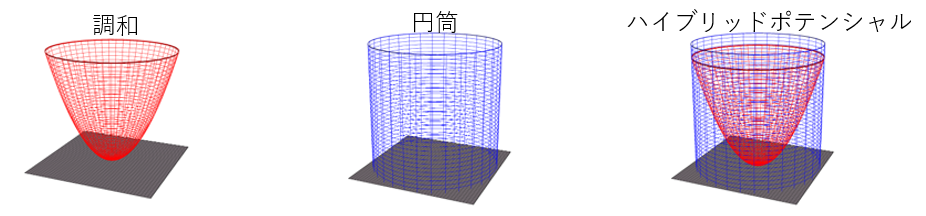
\includegraphics[width=0.4\textwidth]{images/三種盛り.png}

図2.2:量子ドットのポテンシャル
\end{center}
\end{frame}

\section{差分法による解析}
\begin{frame}{4. 実空間差分法}
1次元中心差分:
\[
\left. \frac{d^2 \psi}{dx^2} \right|_{x = i\Delta x}
\approx \frac{\psi_{i+1} - 2\psi_i + \psi_{i-1}}{(\Delta x)^2}
\]

\begin{center}
  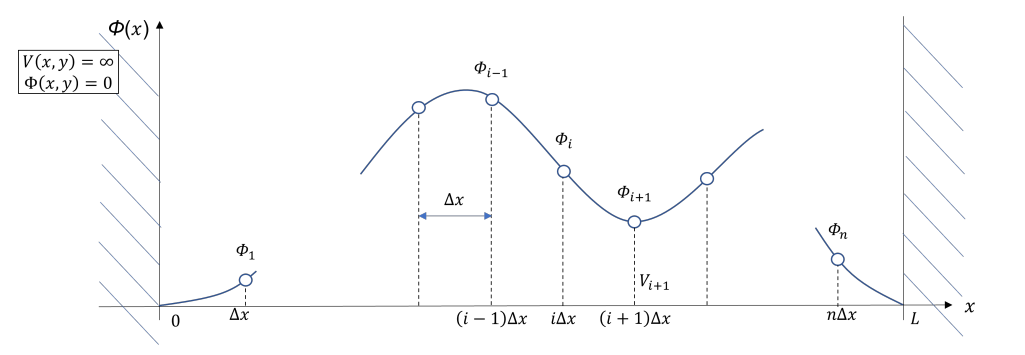
\includegraphics[width=0.65\textwidth]{images/一次元.png}
  
  図4.1:実空間差分法
\end{center}
\end{frame}

\begin{frame}{4.2 2次元差分方程式}
2次元差分ラプラシアン:
\[
\nabla^2 \phi_{i,j} \approx \frac{\phi_{i+1,j} + \phi_{i-1,j} + \phi_{i,j+1} + \phi_{i,j-1} - 4\phi_{i,j}}{(\Delta x)^2}
\]

差分シュレディンガー方程式:
\[
-\frac{1}{2\Delta x^2} (\phi_{i+1,j} + \phi_{i-1,j} + \phi_{i,j+1} + \phi_{i,j-1} - 4\phi_{i,j}) + V_{i,j} \psi_{i,j} = E \psi_{i,j}
\]

\begin{flushright}
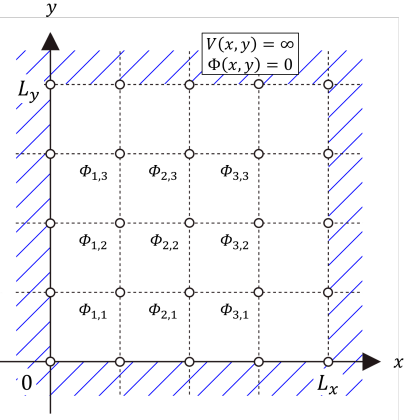
\includegraphics[width=0.3\textwidth]{images/二次元.png}
\end{flushright}
\end{frame}

\begin{frame}{4.3 固有値問題への帰着}
\scriptsize
3x3格子例の行列形式:
\[
-\frac{1}{2\Delta x^2}
\begin{bmatrix}
-4+V_{1,1} & 1 & 0 & \cdots \\
1 & -4+V_{1,2} & 1 & \cdots \\
\vdots & \ddots & \ddots & \ddots
\end{bmatrix}
\bm{\phi}
=
E \bm{\phi}
\]

\begin{center}
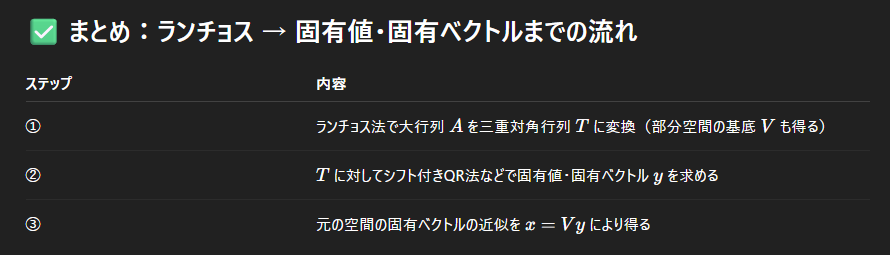
\includegraphics[width=0.6\textwidth]{images/アルゴリズム.png}

図4.1:対角化アルゴリズム
\end{center}
\end{frame}

\section{計算結果の解析}
\begin{frame}{5.1 課題1}
解析解と比較:

\begin{multicols}{3}
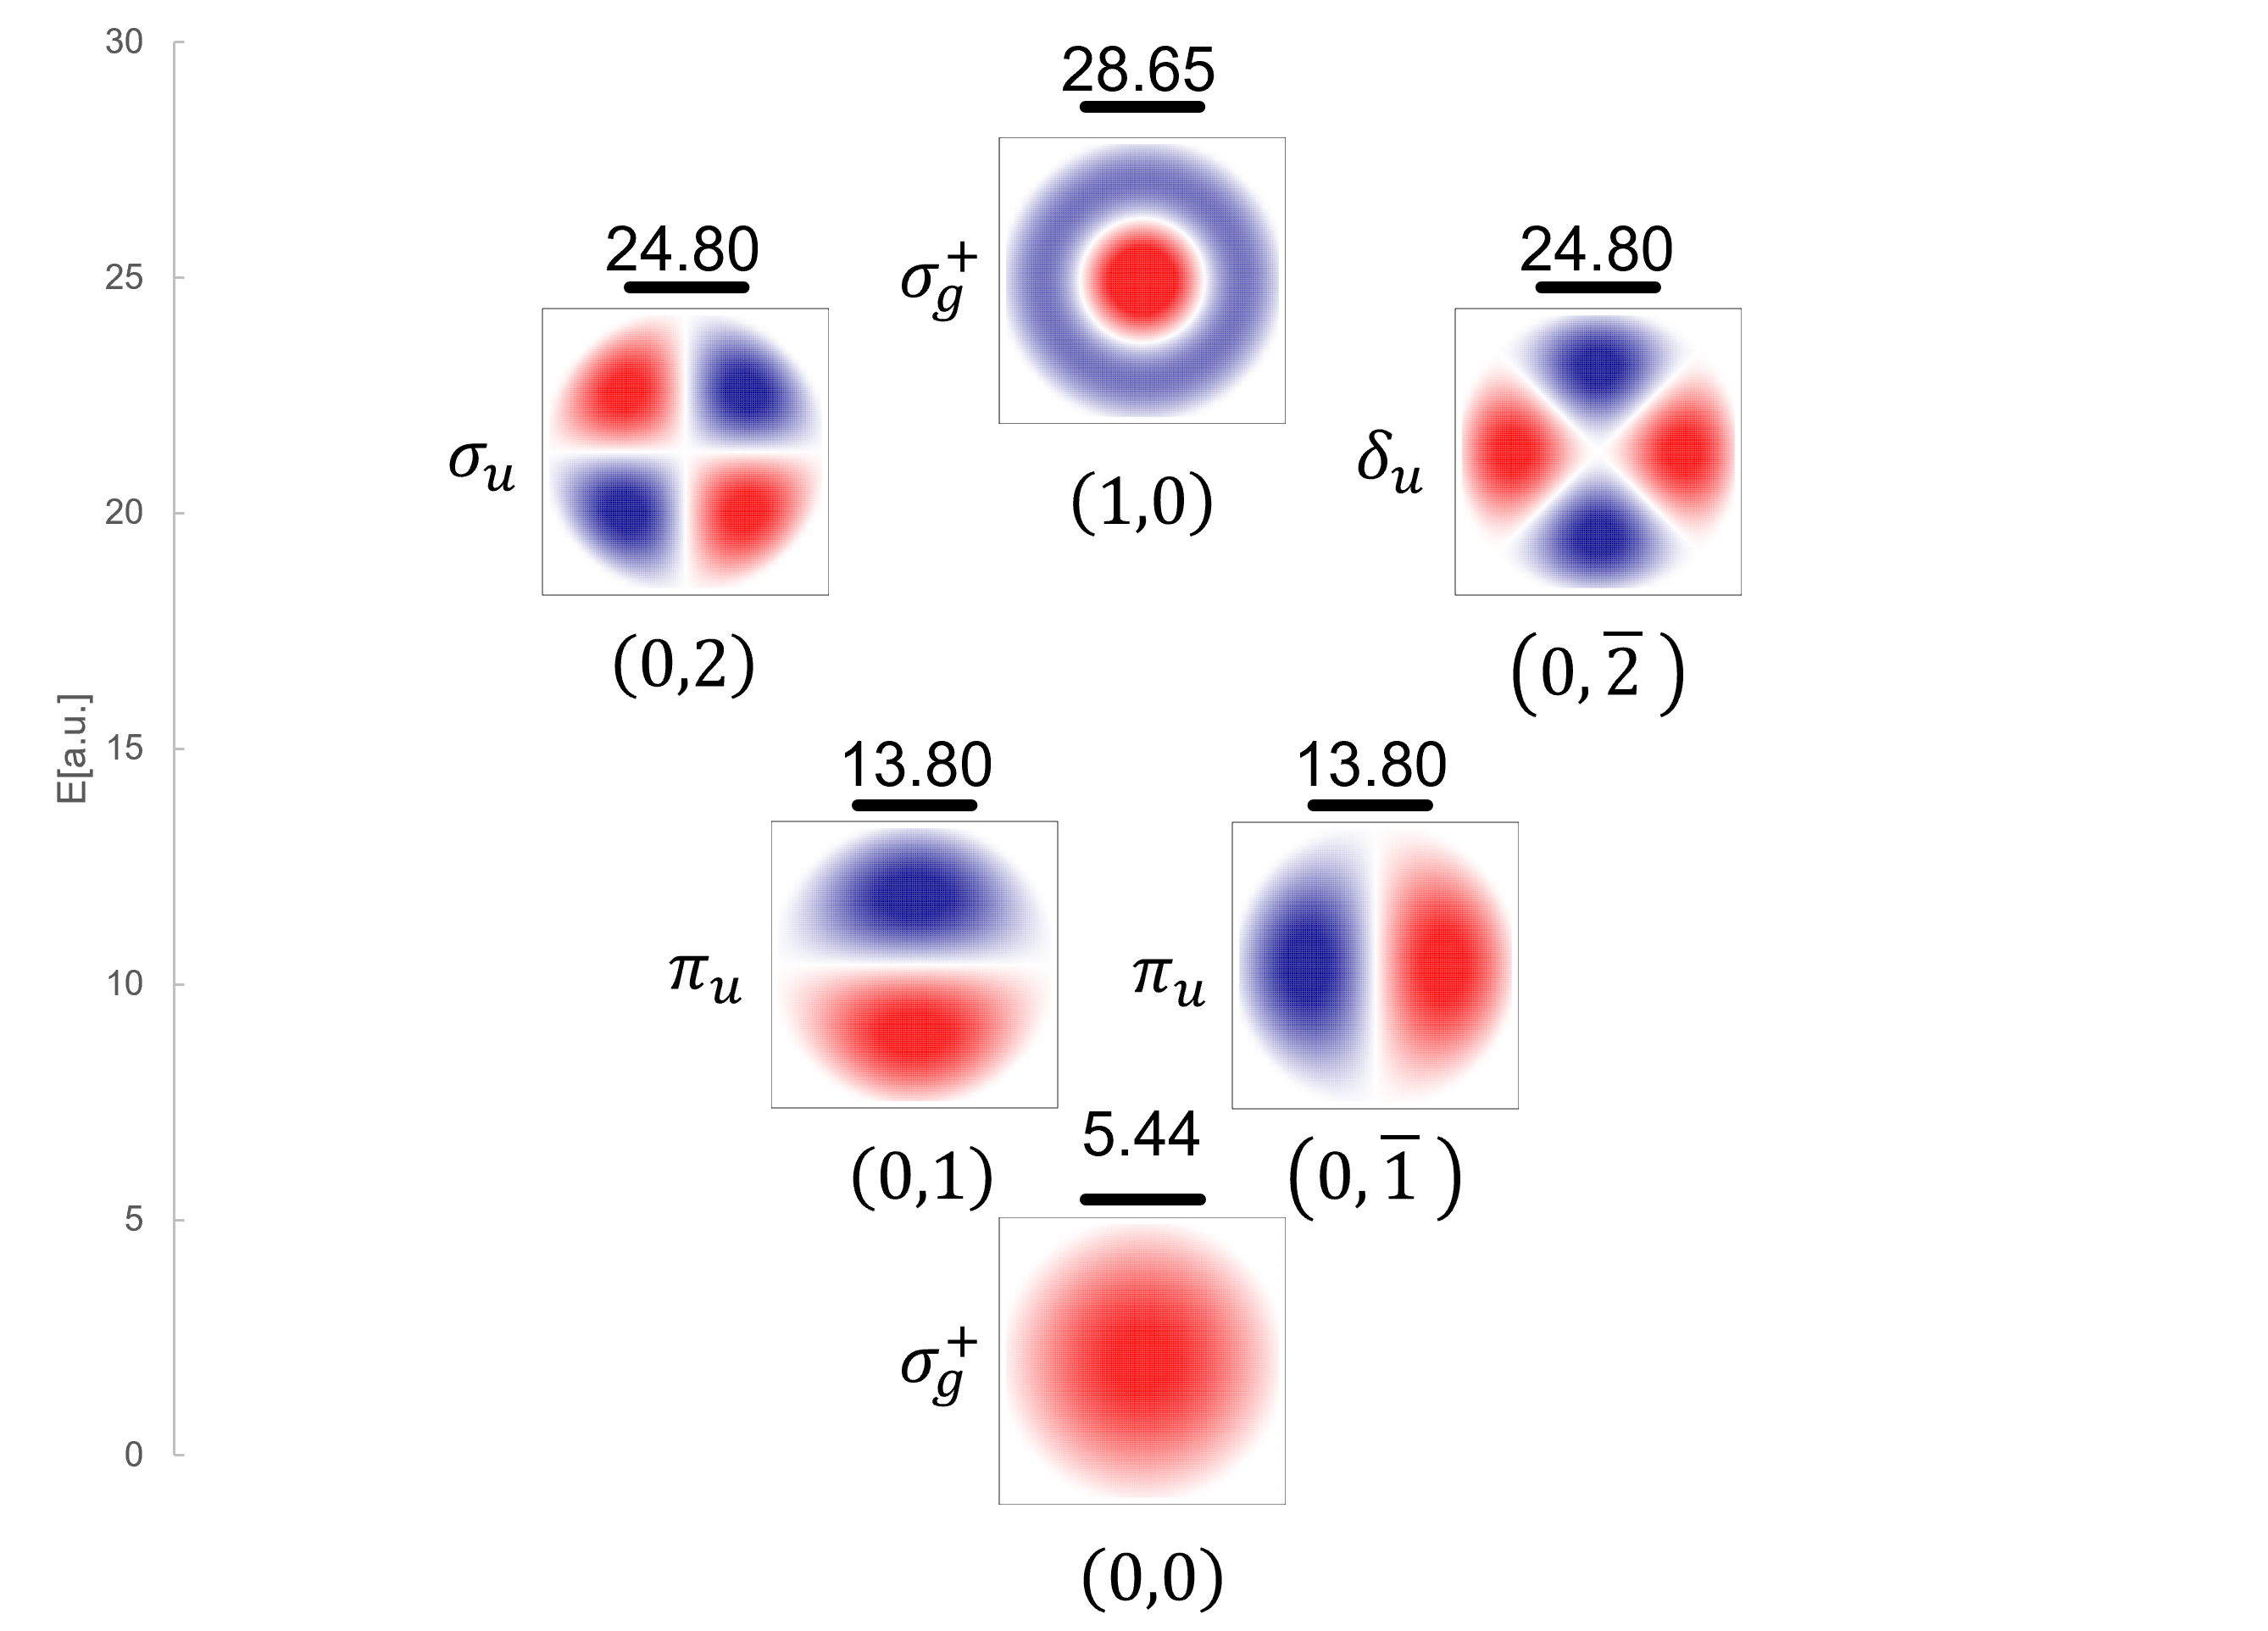
\includegraphics[width=\linewidth]{images/円筒準位図.png}
\centering 図1

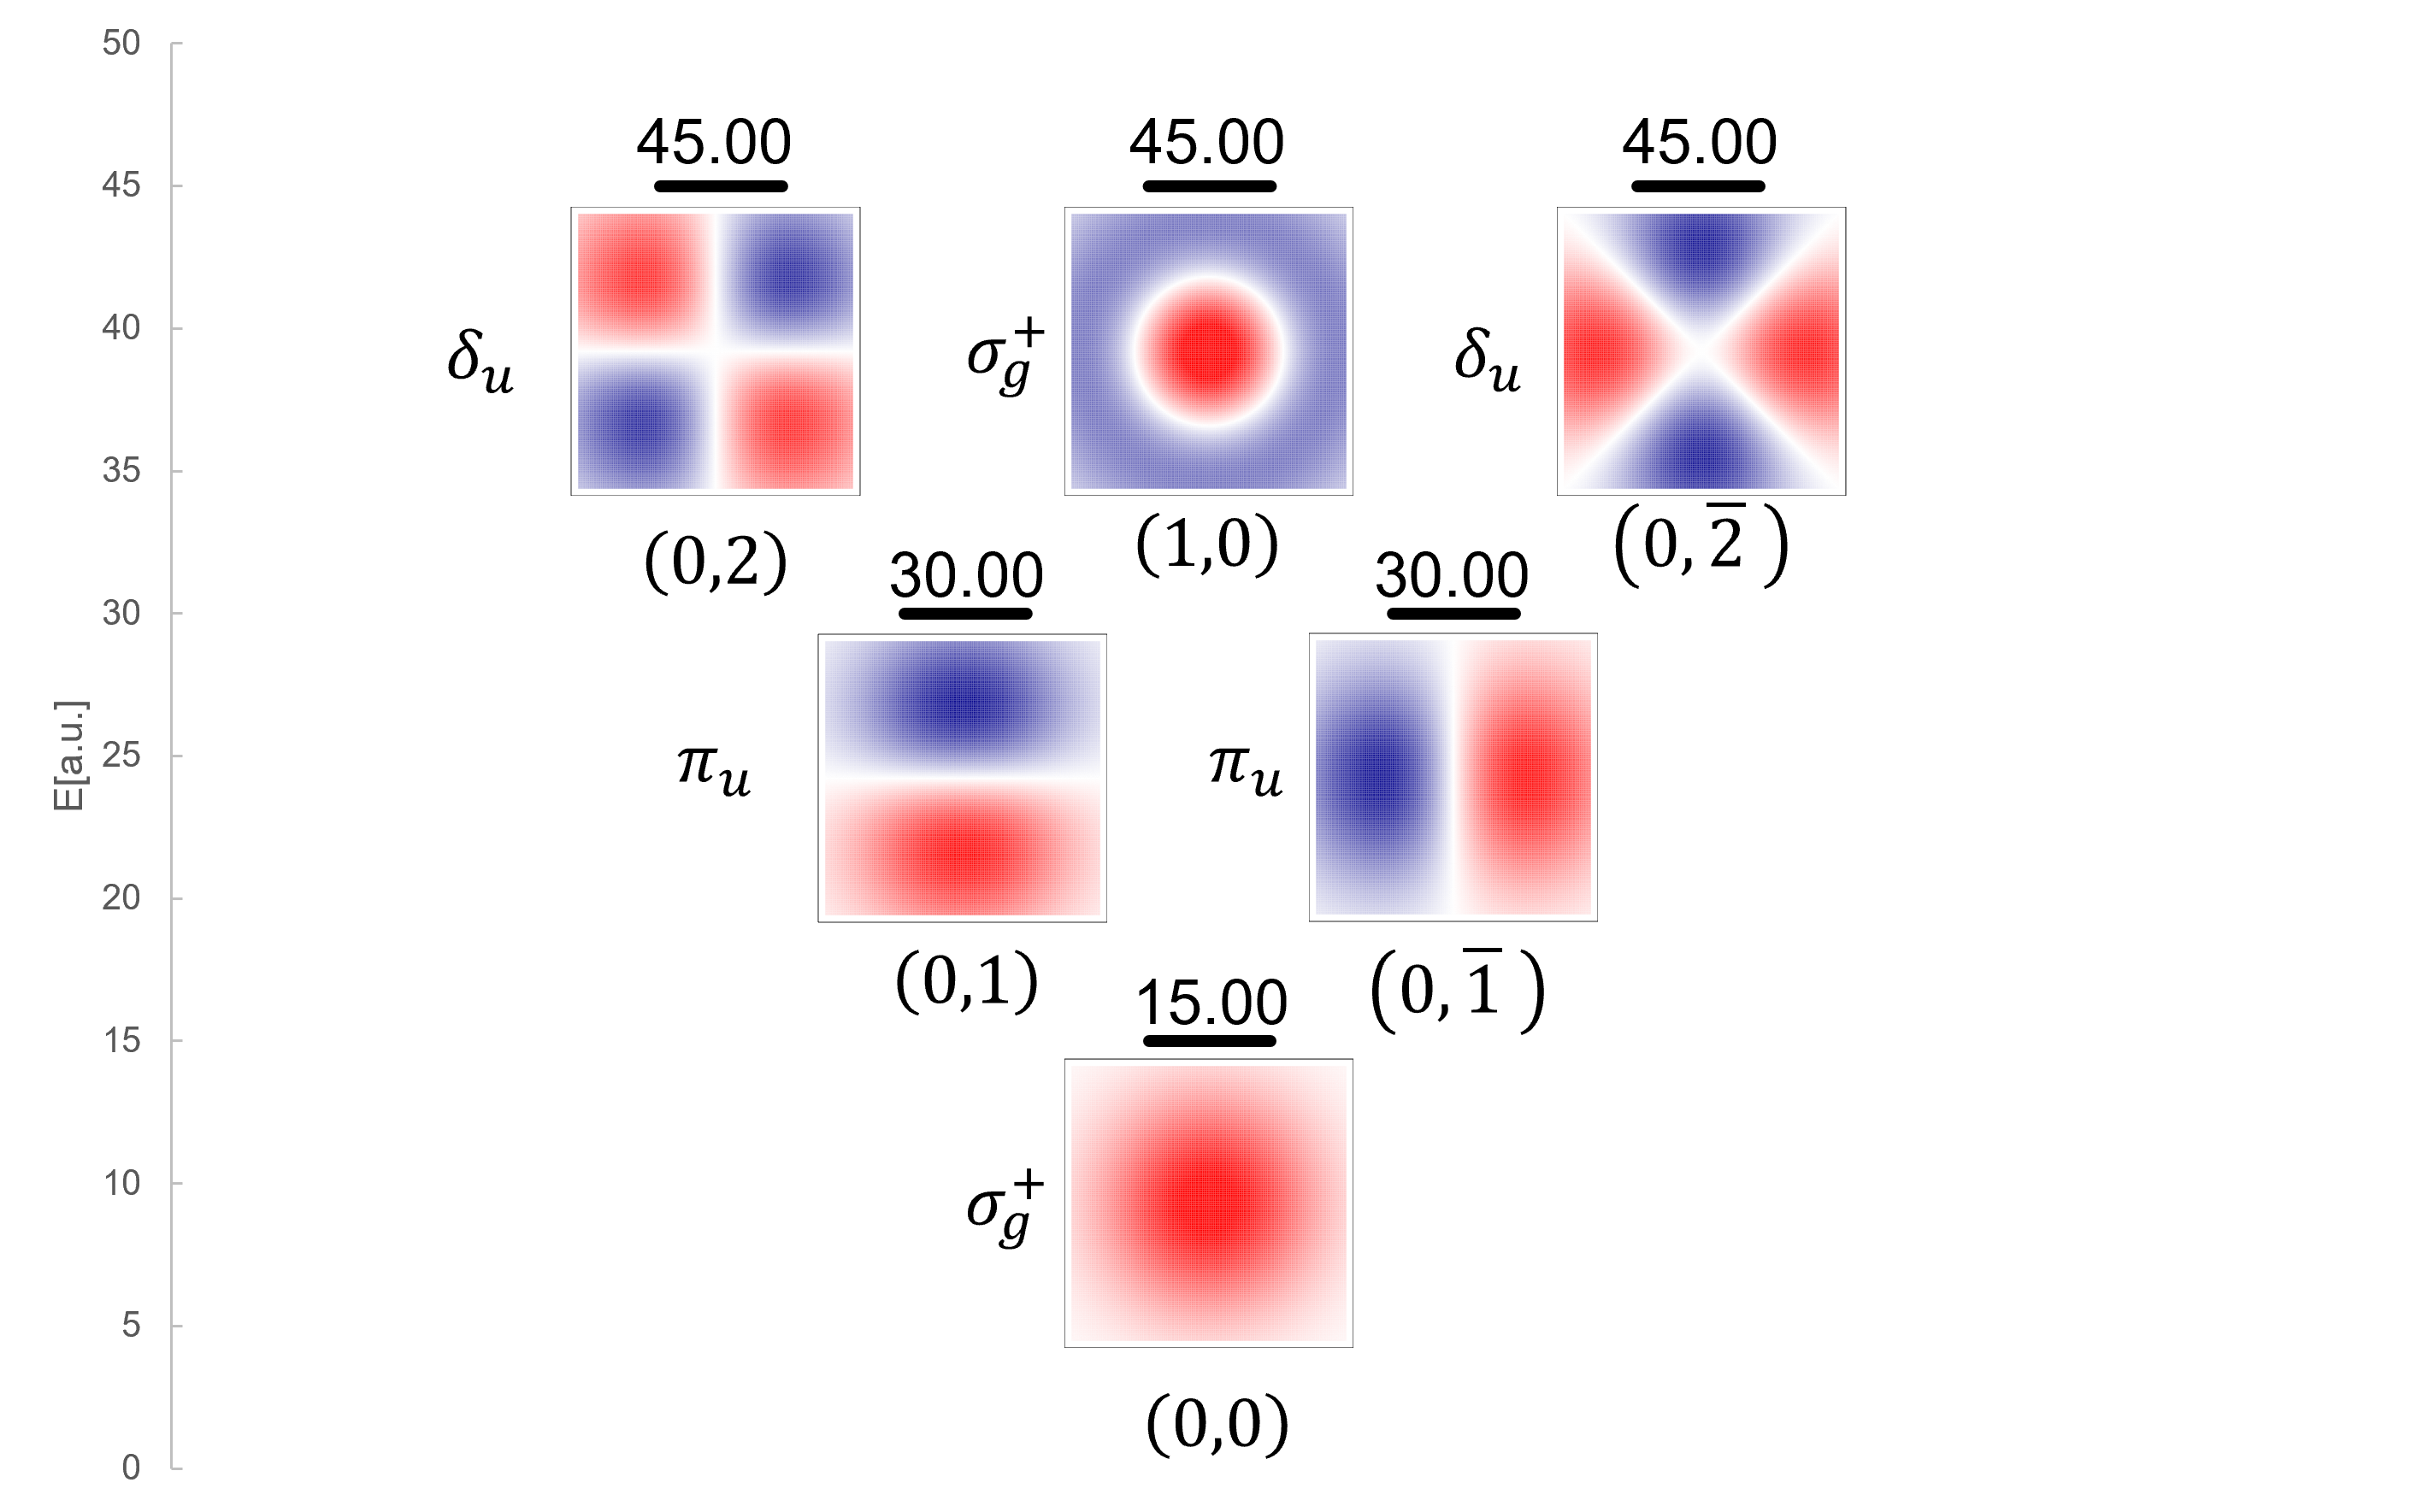
\includegraphics[width=\linewidth]{images/調和準位図.png}
\centering 図2

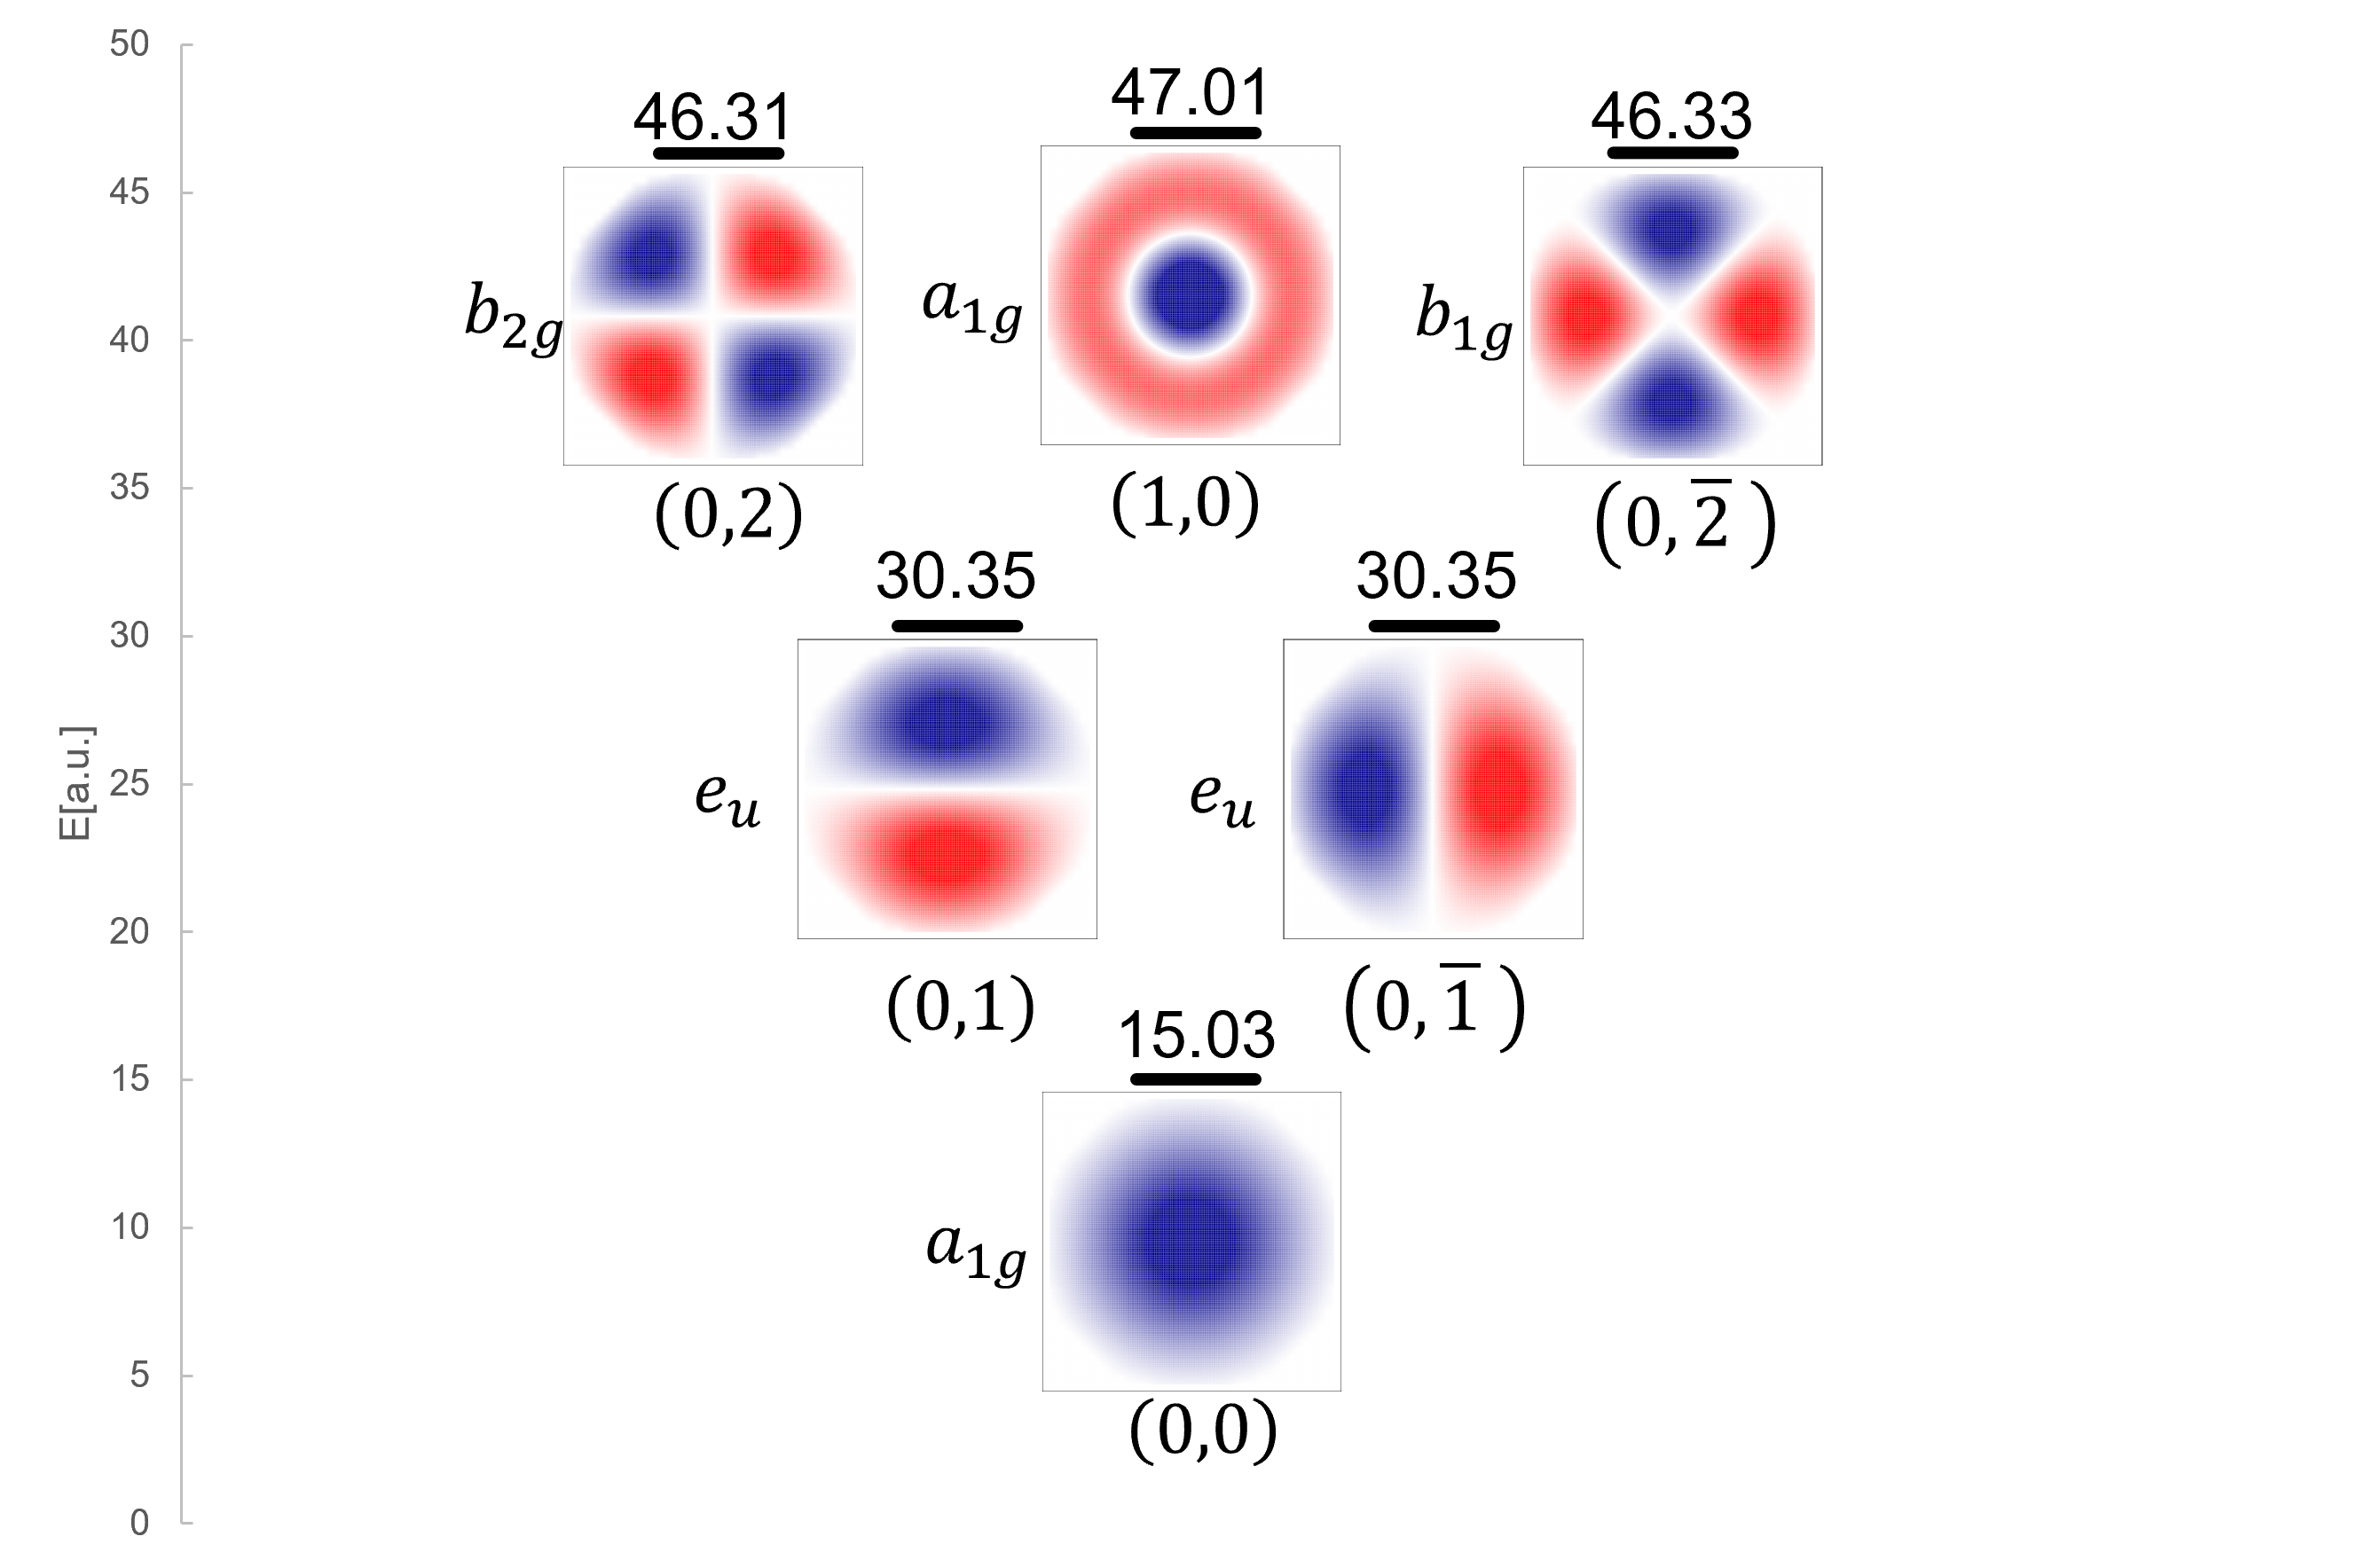
\includegraphics[width=\linewidth]{images/ハイブリッド準位図.png}
\centering 図3
\end{multicols}
\end{frame}


\begin{frame}{5.2 課題2}
閉じ込め強度 $\omega$ を変化させたときのエネルギー準位の比較:

\begin{center}
\includegraphics[width=0.6\textwidth]{images/ωE.svg}

エネルギーの閉じ込め強度依存性
\end{center}
\end{frame}

\end{document}
